\documentclass[12pt,oneside,a4]{article}
\usepackage{float}
\usepackage[utf8]{inputenc}
\usepackage[a4paper,width=160mm,top=25mm,bottom=25mm]{geometry}
\usepackage[lining,tabular]{fbb} % so math uses tabular lining figures
\usepackage{graphicx}
\usepackage{enumitem}
\usepackage{listings}
\usepackage[svgnames]{xcolor}
\usepackage{subfig}

\setlist{leftmargin=*}
\usepackage{listings}
\lstset{basicstyle=\ttfamily,frame=single,xleftmargin=3em,xrightmargin=3em}
\usepackage[os=win]{menukeys}
\renewmenumacro{\keys}[+]{shadowedroundedkeys}
\usepackage{framed}
\usepackage{etoolbox}
\AtBeginEnvironment{leftbar}{\sffamily\small}
\usepackage{array,lipsum}
\newenvironment{fulltable}[1][H]
 {\begin{table}[#1]%
  \hspace*{-\leftmarginwidth}%
  \begin{minipage}{\fullwidth}}
 {\end{minipage}\end{table}}
\usetikzlibrary{chains,arrows,shapes,positioning}
\usepackage{hyperref}
\graphicspath{{figures/}} %Setting the graphicspath
\renewcommand\abstractname{Introduction}




\title{Marble -- Factory Acceptance Tests\\ \small{v1.0 2020}}
\author{Michał Gąska, michalgaska2@gmail.com}

\begin{document}

\maketitle
\begin{center}
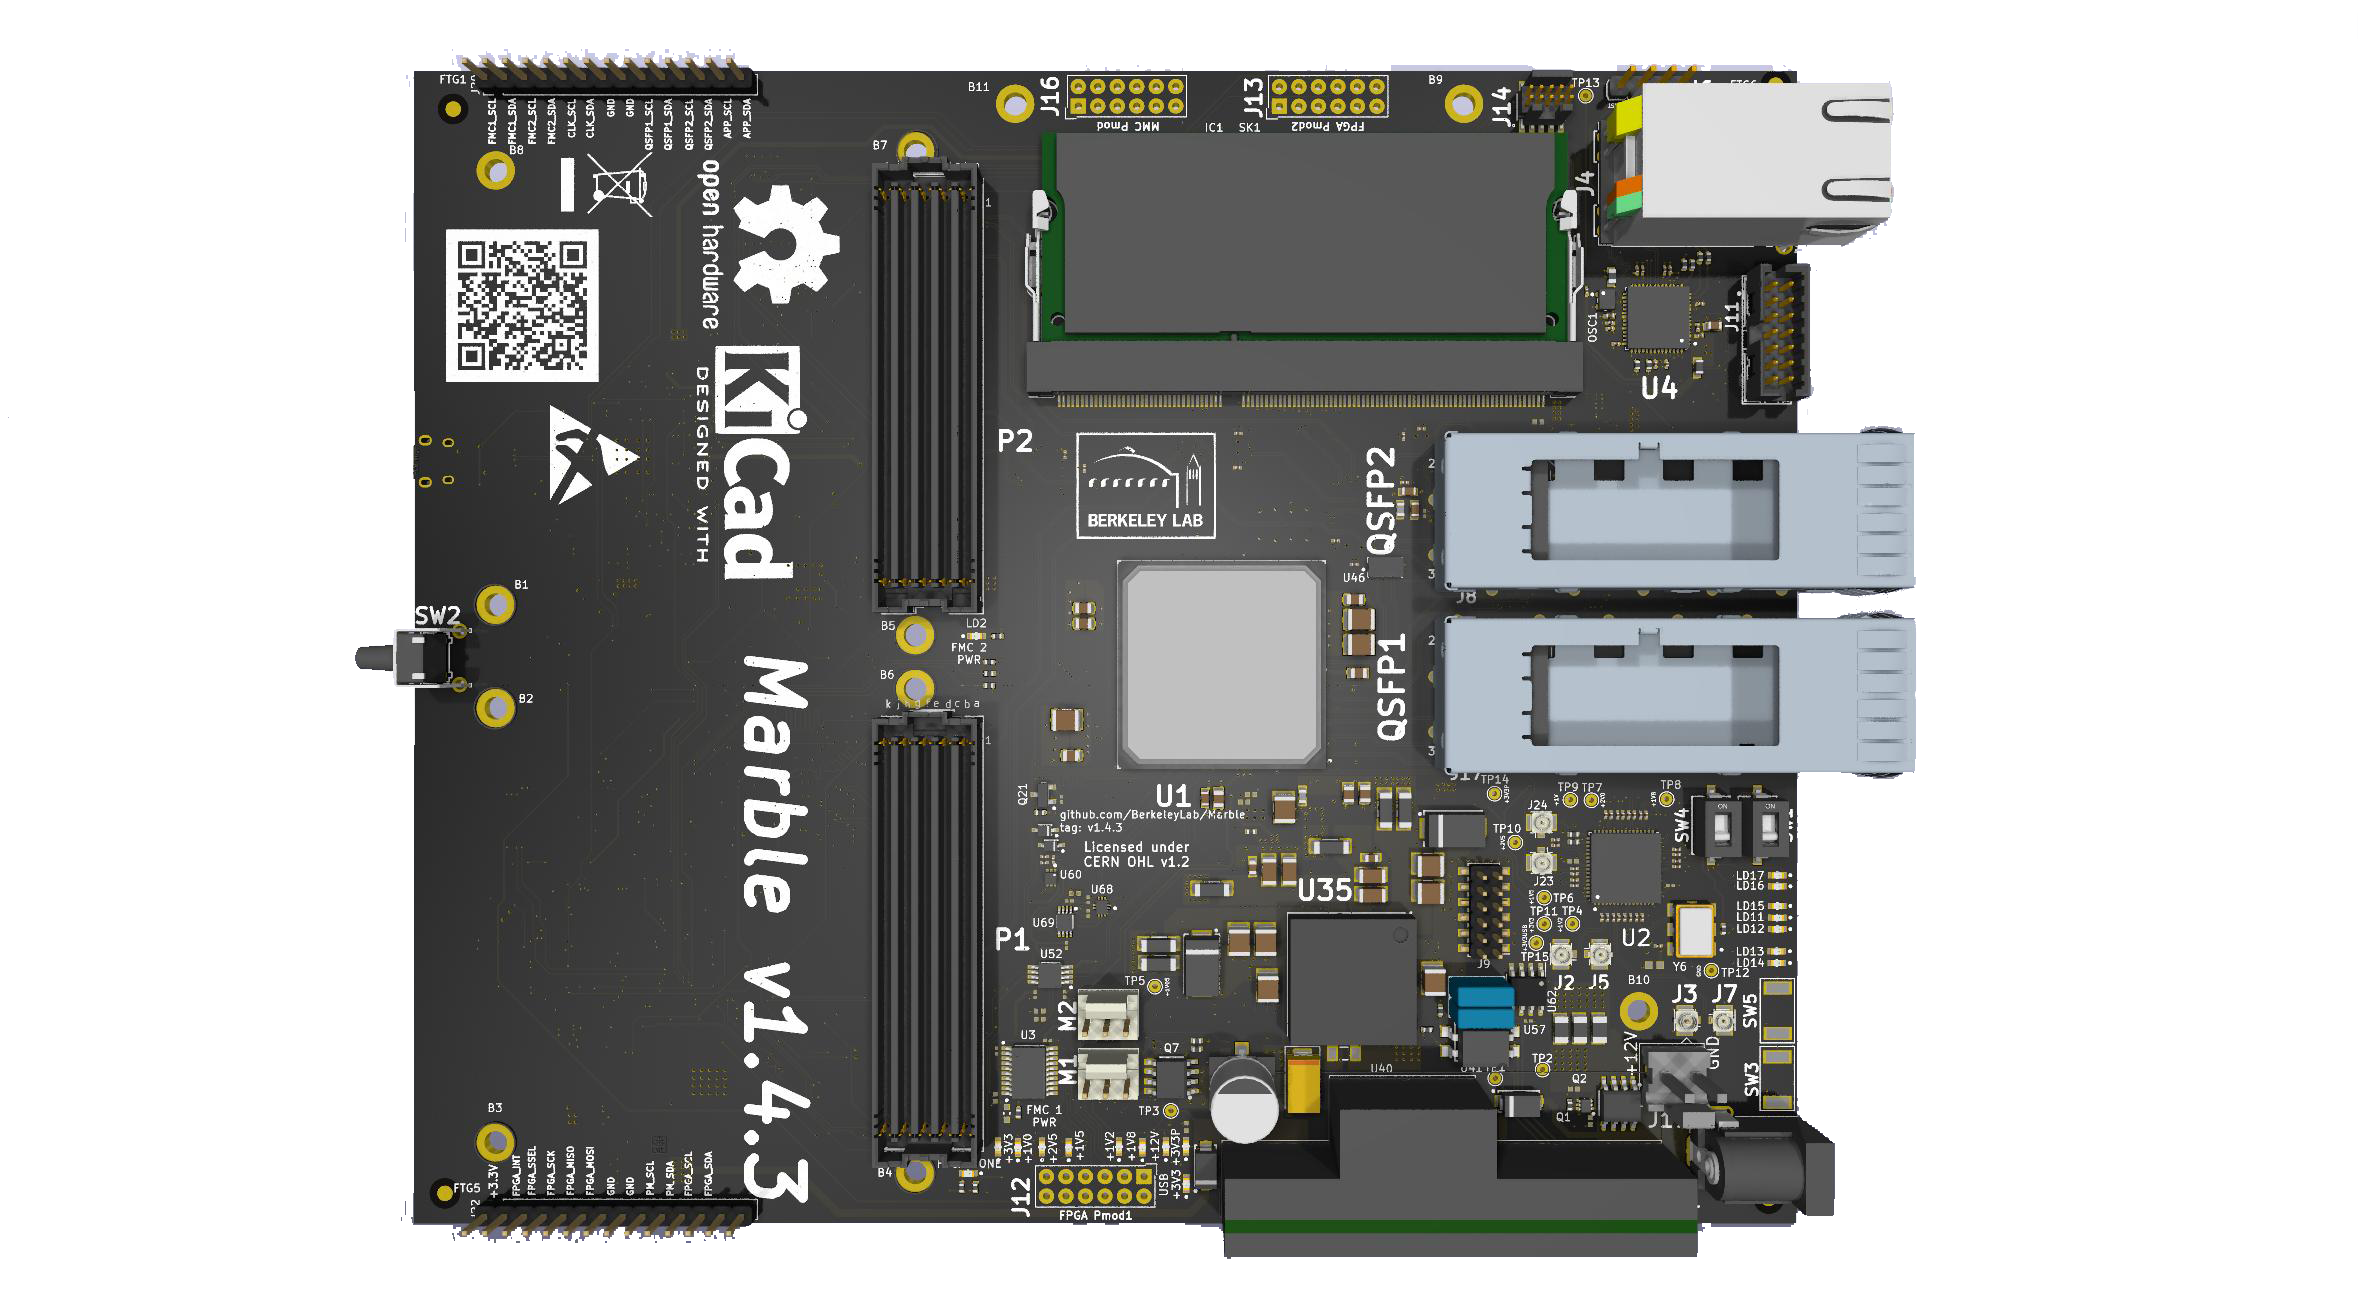
\includegraphics[width=0.8\linewidth]{marble_top.png}
\end{center}
\begin{abstract}
%\includegraphics[width=1.0\linewidth]{PhysLogger.png}\\
This document presents a user--friendly guide on how to perform Factory Acceptance Tests (FAT) for the Marble module. Tests begin from a short description of where Marble's useful connector, LED indicators, and test points are placed on the board. It is highly recommended to perform the tests in the order presented in this document.
\end{abstract}

\clearpage
\tableofcontents

\clearpage

\section{Overview to Marble module}

\begin{leftbar}
Design files are open source and can be downolad from Gilhub:

https://github.com/BerkeleyLab/Marble
\end{leftbar}


\begin{leftbar}
Each board is marked with a revision number. Make sure that the

downloaded files correspond to your board.
\end{leftbar}

\subsection{Hardware requirements}
To perform all of the tests following hardware are required:
\begin{enumerate}
    \item Lab bench power supply.
    \item Micro USB calbe.
    \item QSFP loopback module. 
    \item FMC Tester module. 
    \item Multimeter. 
    \item MMC JTAG (example: SEGGER J-LINK mini).
    \item FPGA JTAG (example: Digilent JTAG HS3).   
\end{enumerate}

\subsection{Software requirements}
To perform all of the tests following software are required:
\begin{enumerate}
    \item Vivado 19.1.
    \item Serial port terminal. 
\end{enumerate}

\section{Power connection}
Before connecting the power supply for the first time, check that the main bus is not shorted. Using a multimeter set in resistance measurement mode, measure the resistance between metal pads of the J19 connector (Figure \ref{01}). 
\begin{figure}[H]
\begin{center}
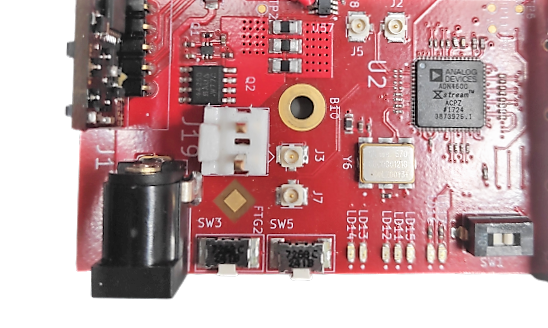
\includegraphics[width=0.9\linewidth]{J19.png}
 \caption{Connector's terminals. }\label{01}
\end{center}
\end{figure}
\begin{leftbar}
Measured resistance should be around \textbf{{\color{red}200 kOhm}}
\end{leftbar}

If the resistance is correct, connect the main power. For this purpose, the current limitation on the power supply should be set to 100mA and the voltage to 12V. \textbf{Make sure that the current limit of the laboratory power supply is on.} Now the power cable can be connected to the board and the used laboratory power supply channel can be switched on. 
This should result in the \textit{12V} LED lighting up as shown  on Figure \ref{02}. Now it is recommended to go to section \nameref{microcontroller}. 
\begin{figure}[H]
\begin{center}
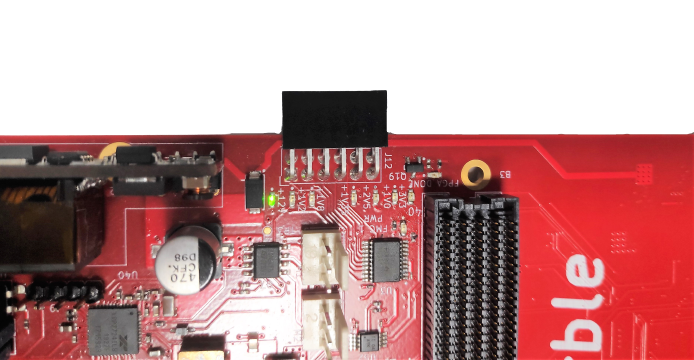
\includegraphics[width=0.8\linewidth, angle = 180]{xrpoff.png}
 \caption{12V indicator LED is on. }\label{02}
\end{center}
\end{figure}

\section{Microcontroller programing}
\label{microcontroller}

Download the latest version of the microcontroller testing code from github:
\begin{leftbar}
https://https://gitlab.lbl.gov/spaiagua/marble\_mmc/-/tree/i2c\_rework
\end{leftbar}

A recent version of OpenOCD (v0.10.0 or later) is required. 
\begin{enumerate}
	\item Connect JTAG module to \textbf{J14} like it is shown on Figure \ref{23}.
	\item Connect the micro USB cable and using the serial terminal, connect to the last serial port for the new listed in the operating system. Use 115200 boudrate.
	\item Power up the board.
	\item Program the microcontroller using the following commands:
	\begin{enumerate}
	\item Go to the main folder of the downloaded repository.
	\item Open command terminal and run command:
	\begin{lstlisting}[backgroundcolor = \color{Gainsboro}, language=bash, frame=none]]
$ make download
	\end{lstlisting}
	\end{enumerate}
	\item After the successful programming, a menu in the serial terminal should appeared and LEDs (LD15, LD11, LD12) should blink in the "snake" pattern.
\end{enumerate}

\begin{figure}[H]
\begin{center}
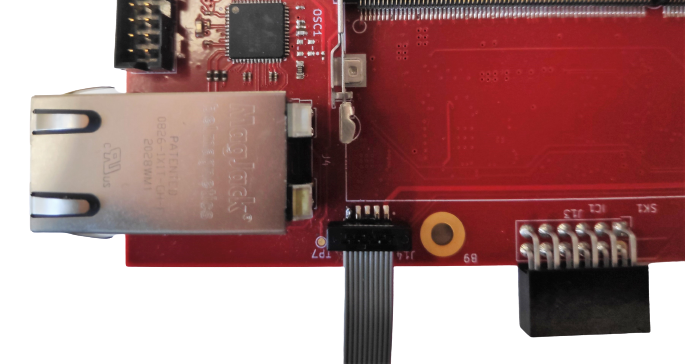
\includegraphics[width=0.8\linewidth]{mmcjtag.png}
 \caption{J14 connector. }\label{23}
\end{center}
\end{figure}



\section{Power Supply programing}
Before doing the steps below, it is highly recommended to measure if there are no shorts on power rails. Measure resistance between the test points:

\begin{enumerate}
    \item \textbf{TP12 (GND)} and \textbf{TP7 (+2V0)}.
    \item \textbf{TP12 (GND)} and \textbf{TP9 (+1V0)}.
    \item \textbf{TP12 (GND)} and \textbf{TP10 (+2V5)}.
    \item \textbf{TP12 (GND)} and \textbf{TP8 (+1V8)}.
    \item \textbf{TP12 (GND)} and \textbf{TP6 (+1V5)}.
    \item \textbf{TP12 (GND)} and \textbf{TP4 (+1V2)}.
    \item \textbf{TP12 (GND)} and \textbf{TP11 (+3V3)}.
    \item \textbf{TP12 (GND)} and \textbf{TP11 (+3V3USB)}.
    \item \textbf{TP12 (GND)} and \textbf{TP11 (+3V3P)}.
    \item \textbf{TP12 (GND)} and \textbf{TP5 (+1V05)}.
\end{enumerate}

\begin{figure}[H]
\begin{center}
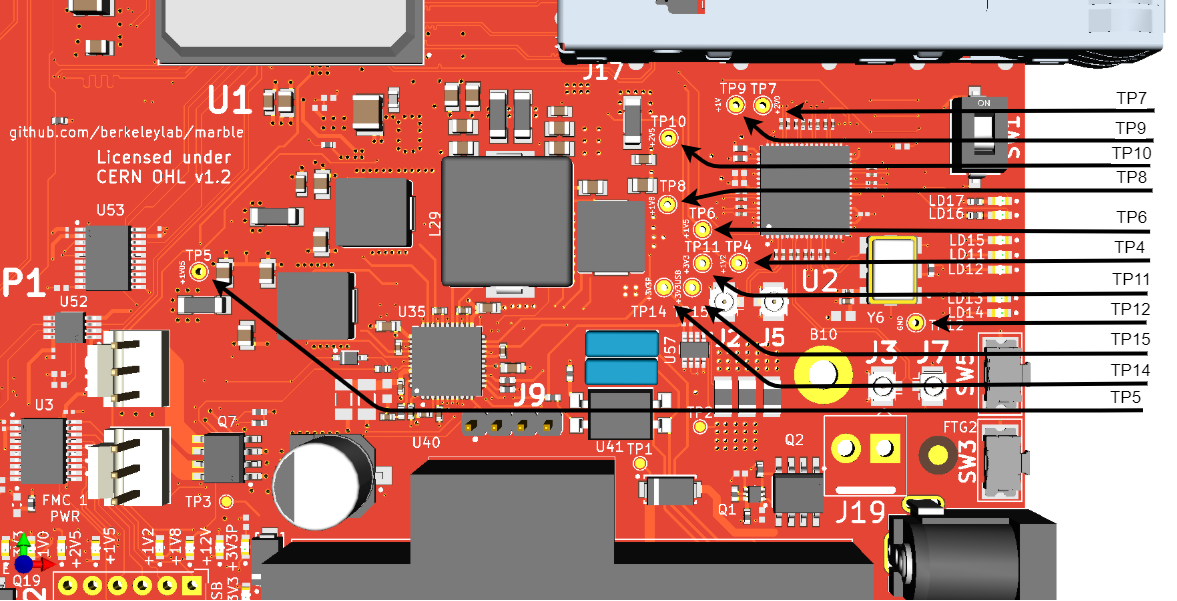
\includegraphics[width=1\linewidth]{Marble_TP.png}
 \caption{Test points. }\label{tp}
\end{center}
\end{figure}

Perform the following steps only and exclusively when there are no shorts on the power rails!
\begin{enumerate}
    \item Connect the micro USB cable and using the serial terminal, connect to the last serial port for the new listed in the operating system. Use 115200 boudrate.
    \item Set up votage to 12V and the current limit to 1A on lab power supply.
    \item Power up the board.
    \item From the menu displayed in the serial terminal, select the option \menu{g) XRP7724 go}.
    \item Make a power cycle by turning off and on the lab power supply.
    \item All power LED indicators should be on (Figure \ref{leds}).
    \item Using multimeter measure voltage between points:
    \begin{enumerate}
    	\item \textbf{TP12 (GND)} and \textbf{TP7 (+2V0)} - expected voltage: +2.0V.
    	\item \textbf{TP12 (GND)} and \textbf{TP9 (+1V0)} - expected voltage: +1.0V.
    	\item \textbf{TP12 (GND)} and \textbf{TP10 (+2V5)} - expected voltage: +2.5V.
    	\item \textbf{TP12 (GND)} and \textbf{TP8 (+1V8)} - expected voltage: +1.8V.
    	\item \textbf{TP12 (GND)} and \textbf{TP6 (+1V5)} - expected voltage: +1.5V.
    	\item \textbf{TP12 (GND)} and \textbf{TP4 (+1V2)} - expected voltage: +1.2V.
    	\item \textbf{TP12 (GND)} and \textbf{TP11 (+3V3)} - expected voltage: +3.3V.
    	\item \textbf{TP12 (GND)} and \textbf{TP11 (+3V3USB)} - expected voltage: +3.3V.
    	\item \textbf{TP12 (GND)} and \textbf{TP11 (+3V3P)} - expected voltage: +3.3V.
    	\item \textbf{TP12 (GND)} and \textbf{TP5 (+1V05)} - expected voltage: +1.05V.
\end{enumerate}
\end{enumerate}

\begin{figure}[H]
\begin{center}
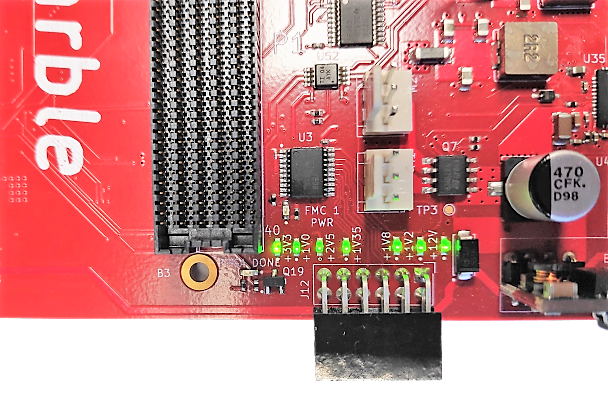
\includegraphics[width=0.7\linewidth]{leds.png}
 \caption{Power LED indicators after a successful power cycle.}\label{leds}
\end{center}
\end{figure}

\section{FPGA programing}
Download the latest version of the FPGA testing code from github:
\begin{leftbar}
https://github.com/BerkeleyLab/Bedrock/tree/marblev2
\end{leftbar}

\begin{leftbar}
Before testing the FPGA it is recommended to set up the current limit to 2A on the lab power supply. 
\end{leftbar}
\subsection{FMC test}
\begin{leftbar}
Board power should be turned off when inserting and removing the FMC module.
\end{leftbar}
\begin{enumerate}
	\item Plug FMC Tester module to one of the FMC connector as it is shown on Figure \ref{fig:example}.
	\item Connect the micro USB cable and using the serial terminal, connect to the last serial port for the new listed in the operating system. Use 115200 boudrate.
	\item Change the network adapter settings to connect with static \textbf{192.168.9.10} IP address.
    \item Connect Marble to the computer using an ethernet cable.
    \item Power up the board.
    \item In the serial terminal menu choose \menu{4) GPIO control
>a) FMC power} to turn on power for FMCs.
	\item Program the FPGA using the following steps:
	\begin{enumerate}
	\item Go to the folder \textbf{Bedrock/projects/test\_marble\_family/}
	\item Open command termianal and run command: 
	\begin{lstlisting}[backgroundcolor = \color{Gainsboro}, language=bash, frame=none]]
$ mutil usb
	\end{lstlisting}
	\end{enumerate}
	\item To make a test do the following steps:
	\begin{enumerate}	
	\item Go to the folder \textbf{Bedrock/projects/test\_marble\_family/}
	\item To test P1 FMC connector run the following command:
	\begin{lstlisting}[backgroundcolor = \color{Gainsboro}, language=bash, frame=none]]
$ PYTHONPATH=../../badger:../../periphera\l_drivers
/i2cbridge python fmc\_test\_c.py --ip $IP --fmc 0
	\end{lstlisting}
	\item To test P2 FMC connector run the following command:
	\begin{lstlisting}[backgroundcolor = \color{Gainsboro}, language=bash, frame=none]]
$ PYTHONPATH=../../badger:../../periphera\l_drivers
/i2cbridge python fmc\_test\_c.py --ip $IP --fmc 1
	\end{lstlisting}
	\end{enumerate}
\end{enumerate}

\begin{figure}[H]%
    \centering
    \subfloat[\centering FMC 1]{{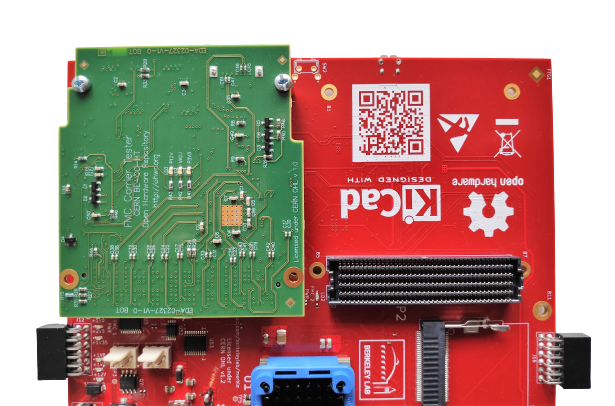
\includegraphics[width=7cm]{fmc1.png} }}%
    \qquad
    \subfloat[\centering FMC 2]{{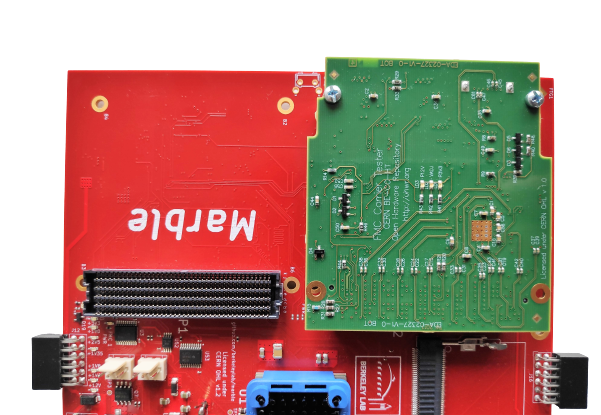
\includegraphics[width=7cm]{fmc2.png} }}%
    \caption{FMC connectors with plugged FMC Tester board.}%
    \label{fig:example}%
\end{figure}

\subsection{QSFP test}

\begin{leftbar}
Board power should be turned off when inserting and removing the QSFP module.
\end{leftbar}
\begin{enumerate}
	\item Plug QSFP loopback module to one of the ports.
	\item Plug FPGA JTAG module.
	\item Configure FPGA using \texttt{marble\_ibert.bit} bit file.
	\begin{enumerate}
		\item Run Vivado
		\item Go to \menu{Flow>Open Hardware Manager} and then  \menu{Tools>Auto Connect}
		\item Click \menu{Tools>Program Device>xc7k160t\_0} to open the programming window. 
		\item Choose the \textit{bitstream file} and click \menu{Program}
	\end{enumerate}
	\item After the successful programming, the Dashboard should start automatically.
	\item Detect links by clicking \menu{Serial I/O Links>Auto-detect links}
	\item Correct detected and working links should look like in figure \ref{links}.  
	\item Connect the QSFP loopback module to the other QSFP connector and repeat the above steps.
\end{enumerate}

\begin{figure}[H]
\begin{center}
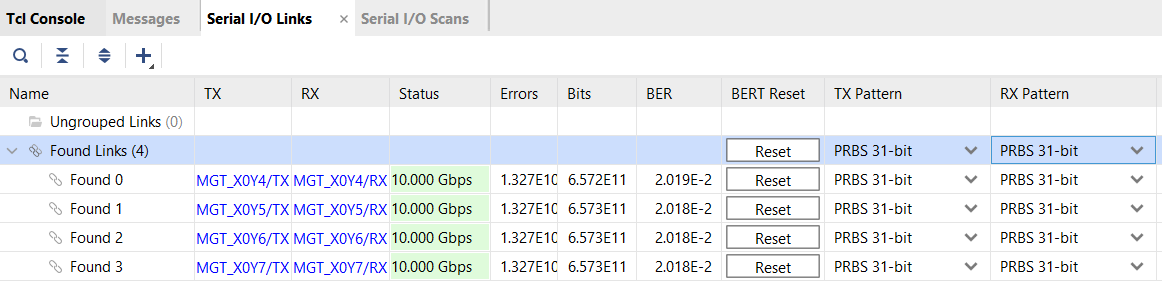
\includegraphics[width=1\linewidth]{links.png}
 \caption{Working links.}\label{links}
\end{center}
\end{figure}

\subsection{Ethernet test}
The following steps should be performed to test the Ethernet:
\begin{enumerate}
    \item Program the FPGA using the following steps:
	\begin{enumerate}
	\item Go to the folder \textbf{Bedrock/projects/test\_marble\_family/}
	\item Open command termianal and run command: 
	\begin{lstlisting}[backgroundcolor = \color{Gainsboro}, language=bash, frame=none]]
$ mutil usb
	\end{lstlisting}
	\end{enumerate}
    \item Change the network adapter settings to connect with static \textbf{192.168.9.10} IP address.
    \item Connect Marble to the computer using an ethernet cable. 
    \item In Linux command terminal run:
    \begin{lstlisting}[backgroundcolor = \color{Gainsboro}, language=bash, frame=none]]
$ ping 192.168.9.10
	\end{lstlisting}
    \item Expected result:
    \begin{lstlisting}[backgroundcolor = \color{Gainsboro}, language=bash, frame=none]]
Pinging [192.168.9.10] with 32 bytes of data:
Reply from 192.168.9.10: bytes=32 time=17ms TTL=55
Reply from 192.168.9.10: bytes=32 time=152ms TTL=55
Reply from 192.168.9.10: bytes=32 time=12ms TTL=55
Reply from 192.168.9.10: bytes=32 time=14ms TTL=55

Ping statistics for 192.168.9.10:
    Packets: Sent = 4, Received = 4, Lost = 0 (0% loss),
Approximate round trip times in milli-seconds:
    Minimum = 12ms, Maximum = 152ms, Average = 48ms
	\end{lstlisting}
    \item For data traffic test use \textit{iperf}. Run command:
    \begin{lstlisting}[backgroundcolor = \color{Gainsboro}, language=bash, frame=none]]
$ iperf -c 192.168.9.10 -u -b 1000M -p 802
	\end{lstlisting}
\end{enumerate}


\section{Appendix}
\subsection{An alternative way to program FPGA}
Programming FPGA using Vivado and Digilent JTAG HS3:
\begin{enumerate}
		\item Run Vivado
		\item Go to \menu{Flow>Open Hardware Manager} and then  \menu{Tools>Auto Connect}
		\item Click \menu{Tools>Program Device>xc7k160t\_0} to open the programming window. 
		\item Choose the \textit{bitstream file} and click \menu{Program}

	\item After the successful programming, the Dashboard should start automatically.
\end{enumerate}
\begin{thebibliography}{99}
%\bibitem{web1} \url{http://bit.ly/PhysLab_Link01}
%\bibitem{web2} \url{http://bit.ly/PhysLab_Link02}
\end{thebibliography}
\end{document}